\documentclass{beamer}
%\documentclass[handout]{beamer}
% This file is a solution template for:

% - Giving a talk on some subject.
% - The talk is between 15min and 45min long.
% - Style is ornate.

% Copyright 2004 by Till Tantau <tantau@users.sourceforge.net>.
%
% In principle, this file can be redistributed and/or modified under
% the terms of the GNU Public License, version 2.
%
% However, this file is supposed to be a template to be modified
% for your own needs. For this reason, if you use this file as a
% template and not specifically distribute it as part of a another
% package/program, I grant the extra permission to freely copy and
% modify this file as you see fit and even to delete this copyright
% notice. 


\mode<presentation>
{
  \usetheme{Montpellier}

  %\setbeamercovered{transparent}
  % or whatever (possibly just delete it)
}

\usepackage{xmpmulti} % package that defines \multiinclude

\usepackage[english]{babel}

\usepackage[latin1]{inputenc}

\usepackage{times}
\usepackage[T1]{fontenc}
% Or whatever. Note that the encoding and the font should match. If T1
% does not look nice, try deleting the line with the fontenc.

\title [Vovk's algorithm] %(optional, use only with long paper titles)
{Vovk's aggregating algorithm \\ Mixable and unmixable loss functions}
\author[Freund] % (optional, use only with lots of authors)
{Yoav Freund}
% - Give the names in the same order as the appear in the paper.
% - Use the \inst{?} command only if the authors have different
%   affiliation.

\institute[Universities of Somewhere and Elsewhere] % (optional, but mostly needed)

\subject{Machine Learning}
% This is only inserted into the PDF information catalog. Can be left
% out. 

% If you have a file called "university-logo-filename.xxx", where xxx
% is a graphic format that can be processed by latex or pdflatex,
% resp., then you can add a logo as follows:

% \pgfdeclareimage[height=0.5cm]{university-logo}{university-logo-filename}
% \logo{\pgfuseimage{university-logo}}



% Delete this, if you do not want the table of contents to pop up at
% the beginning of each subsection:
%% \AtBeginSubsection[]
%% {
%%   \begin{frame}<beamer>
%%     \frametitle{Outline}
%%     \tableofcontents[currentsection,currentsubsection]
%%   \end{frame}
%% }


% If you wish to uncover everything in a step-wise fashion, uncomment
% the following command: 

\beamerdefaultoverlayspecification{<+->}

\newcommand{\newmcommand}[2]{\newcommand{#1}{{\ifmmode {#2}\else\mbox{${#2}$}\fi}}}
\newcommand{\renewmcommand}[2]{\renewcommand{#1}{{\ifmmode {#2}\else\mbox{${#2}$}\fi}}}
\newcommand{\newmcommandi}[2]{\newcommand{#1}[1]{{\ifmmode {#2}\else\mbox{${#2}$}\fi}}}
\newcommand{\newmcommandii}[2]{\newcommand{#1}[2]{{\ifmmode {#2}\else\mbox{${#2}$}\fi}}}
\newcommand{\newmcommandiii}[2]{\newcommand{#1}[3]{{\ifmmode {#2}\else\mbox{${#2}$}\fi}}}

\newcommand{\algfnt}{\bf}

\newmcommand{\ouralg}{{\mbox{\algfnt Hedge}({\eta})}}

\newmcommand{\iter}{T}

\newfont{\cmmib}{cmmib10}
\newcommand{\boldell}{{\mbox{\cmmib \symbol{'140}}}}


\newmcommandi{\costvec}{{\boldell}_{#1}}
\newmcommandii{\cost}{{\ell}^{#1}_{#2}}

\newmcommandi{\rd}{\tilde{#1}}

\newmcommandi{\distvec}{{\bf p}^{#1}}
\newmcommandi{\rddistvec}{\rd{\bf p}^{#1}}
\newmcommandii{\dist}{{p}^{#1}_{#2}}
\newmcommandii{\rddist}{\rd{p}^{#1}_{#2}}

\newmcommandi{\bdistvec}{{\bf q}^{#1}}
\newmcommandii{\bdist}{{q}^{#1}_{#2}}

\newmcommandi{\wtvec}{{\bf w}^{#1}}
\newmcommandi{\rdwtvec}{\rd{\bf w}^{#1}}
\newmcommandii{\wt}{{w}^{#1}_{#2}}
\newmcommandii{\rdwt}{\rd{w}^{#1}_{#2}}


\newcommand{\Nweight}[2]{V_{#1}^{#2}}	%the normalized weight
\newcommand{\dweight}[2]{w^{#2}(#1)} % initial density measure
\newcommand{\TEloss}[1]{L_{#1}}	%total loss of expert i
\newcommand{\BEloss}{L_{\min}}	%total loss of the best expert
\newcommand{\TAloss}{L_A}	%total loss of algorithm
\newcommand{\weight}[2]{W_{#1}^{#2}} % weight assigned to expert
\newcommand{\btheta}{\hat{\theta}}

\newcommand{\R}[1]{{\color{red}{#1}}}
\newcommand{\B}[1]{{\color{blue}{#1}}}
\newcommand{\RM}[1]{{\color{red}{$#1$}}}


%BANDITS
\newcommand{\Aplay}{{\bf Hedge}}
\newcommand{\Aest}{{\bf Exp3}}
\newcommand{\Aesthp}{{\bf Exp3.P}}
\newcommand{\Aestg}{{\bf Exp3.P.1}}
\newcommand{\Aests}{{\bf Exp3.S}}
\newcommand{\Aessg}{{\bf Exp3.S.1}}
\newcommand{\Astrat}{{\bf Exp4}}
\newcommand{\Abound}{{\bf Exp3.1}}
\newcommand{\Gbest}{G_{\rm max}}

\newcommand{\defeq}{\stackrel{\rm def}{=}}
\newcommand{\compl}{\mbox{\sc h}}
\newcommand{\theset}[2]{\{ {#1} \,:\, {#2} \}}

\newmcommandii{\stratv}{\mbox{\boldmath $\xi$}^{#1}({#2})}

%Games paper
\newmcommand{\M}{\bf M}
\newmcommand{\dM}{\M'}
\newmcommand{\Row}{\bf R}
\newmcommand{\dRow}{\R'}
\newmcommand{\C}{\bf C}
\newmcommand{\dC}{\C'}
\newmcommand{\D}{D}
\renewmcommand{\P}{\bf P}
\newmcommand{\Q}{\bf Q}
\newmcommand{\Dt}{\D_t}
\newmcommand{\Pt}{\P_t}
\newmcommand{\Qt}{\Q_t}
\newmcommand{\Pstar}{\P^*}	% the min/max optimal mixed strategy
\newmcommand{\Pref}{\tilde{\P}}	% a reference mixed strategy (not
				% necessarily min/max)
\newmcommand{\Qstar}{\Q^*}
\newmcommand{\Pa}{\overline{\P}}
\newmcommand{\Qa}{\overline{\Q}}
\newmcommand{\Qh}{\hat{\Q}}
\newmcommandi{\trans}{{#1}^{\rm T}}
\newmcommand{\mhx}{\M(h,x)}
\newmcommand{\mxh}{\dM(x,h)}
\newmcommand{\mpq}{\M(\P,\Q)}
\newmcommand{\mpsq}{\M(\Pstar,\Q)}
\newmcommand{\mpsqt}{\M(\Pstar,\Qt)}
\newmcommand{\mptqt}{\M(\Pt,\Qt)}
\newmcommand{\mptt}{\M(\Pt,t)}
\newmcommand{\mptq}{\M(\Pt,\Q)}
\newmcommand{\mpqt}{\M(\P,\Qt)}
\newcommand{\minp}{\min_{\P}}
\newcommand{\maxq}{\max_{\Q}}
\newcommand{\RE}[2]{{\rm RE}\left( {#1} \; \parallel \; {#2} \right) }

\newmcommand{\sumt}{\sum_{t=1}^T}
\newmcommand{\sumin}{\sum_{i=1}^n}
\newmcommand{\delt}{\Delta_{T,n}}
\newcommand{\nextline}{\vspace{0.2cm}\\}   % a little space for equation arrays

\newcommand{\lwalg}{\mbox{\rm MW}}
\newcommand{\lwalgvar}{\mbox{\rm vMW}}

%%
\newcommand{\E}{\mbox{\rm\bf E}}
\newcommand{\p}[2]{p_{#1}(#2)}
\newcommand{\q}[2]{q_{#1}(#2)}
\newcommand{\x}[2]{x_{#1}({#2})}
\newmcommand{\bx}{\mbox{\boldmath$x$}}
\newmcommandi{\xv}{\bx({#1})}
\newmcommand{\xvt}{\xv{t}}
%\newcommand{\w}[2]{w_{#1}({#2})} replaced by \wt, but remember to switch order of parameters i and t
\renewcommand{\i}[1]{i_{#1}}
\newcommand{\hx}[2]{\hat{x}_{#1}(#2)}
\newcommand{\hxit}{\hx{\i{t}}{t}}
\newcommand{\pit}{\p{\i{t}}{t}}
\newcommand{\xit}{\x{\i{t}}{t}}
\newcommand{\expb}[1]{\exp\left(#1\right)}

\newcommand{\vp}{{\mathbf p}}
\newcommand{\vu}{{\mathbf u}}
\newcommand{\vv}{{\mathbf v}}
\newcommand{\vx}{{\mathbf x}}
\newcommand{\vy}{{\mathbf y}}
\newcommand{\vw}{{\mathbf w}}
\newcommand{\vz}{{\mathbf z}}
\newcommand{\vq}{{\mathbf q}}
\newcommand{\vg}{{\mathbf g}}

\newcommand{\vecq}{{\bf q}}
\newcommand{\vecp}{{\bf p}}


\newcommand{\HedgeLoss}{L_{\mbox{\footnotesize Hedge}}}

\newcommand{\W}{\vec{W}}
\newcommand{\V}{\vec{V}}
\newcommand{\X}{\vec{X}}
\newcommand{\vb}{\vec{b}}
%\newcommand{\loss}{\vec{\ell}}
\newcommand{\loss}{L}
\newcommand{\elloss}[2]{\ell_{#2}\left( #1 \right)} %loss of expert i at time t
\newcommand{\lossvec}[1]{{\mathbf \ell}_{#1}}       %loss of expert at time t
\newcommand{\w}[1]{\makebox[12pt]{{#1}}}
\newcommand{\Rps}{\mbox{\tt R}}
\newcommand{\rPs}{\mbox{\tt P}}
\newcommand{\rpS}{\mbox{\tt S}}
\newcommand{\rpstie}{\w{$\frac{1}{2}$}}
\newcommand{\rpswin}{\w{$0$}}
\newcommand{\rpsloss}{\w{$1$}}

\newmcommand{\decspace}{\Delta}
\newmcommand{\decsym}{\delta}
\newmcommandi{\dec}{\decsym^{#1}}
\newmcommand{\decdistsym}{\cal D}
\newmcommandi{\decdist}{{\decdistsym}^{#1}}

\newmcommand{\simpdistspace}{{\bf \cal S}}
\newmcommand{\domset}{{\rm dom}(\decdistsym)}

\newmcommand{\expdistsym}{{\cal E}}
\newmcommandii{\expdist}{{\expdistsym}^{#1}_{#2}}
\newmcommand{\expdecsym}{{\varepsilon}}
\newmcommandii{\expdec}{\expdecsym^{#1}_{#2}}

\newmcommand{\outspace}{\Omega}
\newmcommand{\outsym}{\omega}
\newmcommandi{\out}{\outsym^{#1}}

%\newmcommandii{\Dkl}{D_{\mbox{kl}}\paren{#1||#2}}
\newmcommandii{\Dkl}{{\rm {KL}}\paren{{#1}\;||\;{#2}}}

\newmcommandi{\sumwts}{\sum_{i=1}^N \wt{#1}{i}}

\newmcommand{\lossalg}{L_A}
\newmcommand{\lossouralg}{{L_{\mbox{\scriptsize\algfnt Hedge}(\eta)}}}
\newmcommand{\lossS}{{L_{\mbox{\scriptsize\algfnt S}}}}
\newmcommandi{\lossi}{L_{#1}}
\newmcommandii{\lossit}{L_{#1}^{#2}}

\newmcommandi{\upbnd}{\tilde{#1}}

\newcommand{\angles}[1]{{\left\langle {#1} \right\rangle}}
\newcommand{\paren}[1]{{\left( {#1} \right)}}
\newcommand{\brac}[1]{{\left[ {#1} \right]}}
\newcommand{\braces}[1]{{\left\{ {#1} \right\}}}

\newcommand{\abs}[1]{{\left| {#1} \right|}}
\newcommand{\ceiling}[1]{{\left\lceil {#1} \right\rceil}}

\newfont{\msym}{msbm10}
\newcommand{\real}{\mbox{\msym R}}

\newmcommand{\updatefcn}{U_\eta}

%% \newtheorem{theorem}{Theorem}	
%% \newtheorem{lemma}[theorem]{Lemma}
%% \newtheorem{corollary}[theorem]{Corollary}
%% \newtheorem{definition}{Definition}

%\newcommand{\proof}{\noindent{\bf Proof:} }
%\newcommand{\example}[1]{{\em Example #1.} }
%\newcommand{\qed}{\rule{0.7em}{0.7em}}

\newcommand{\WeakAlg}{\mbox{\algfnt WeakLearn}}
\newcommand{\Boost}{\mbox{\algfnt AdaBoost}}
\newcommand{\EX}{\mbox{\bf EX}}
\newmcommand{\hf}{h_{{f}}}
\newmcommand{\rdhf}{\rd{h}_{{f}}}
\newmcommand{\hfT}{h^T_{{f}}}
\newmcommand{\ranh}{{b}}

\newmcommand{\conclass}{{\cal C}}

\newmcommand{\badvec}{{\bf b}}
\newmcommandi{\bad}{{b}_{#1}}

%%%%%%%% New commands defined for the game-playing paper

\newmcommand{\hedge}{\algfnt Hedge}
\newmcommand{\play}{\algfnt Play}
\newmcommandi{\Glossvec}{{\bg y}^{#1}}
\newmcommandii{\Gloss}{{y}^{#1}_{#2}}
%\newmcommandi{\action}{{I}_{#1}}
\newmcommandi{\Gdistvec}{{\bf \tilde{p}}^{#1}}
\newmcommandii{\Gdist}{{\teilde{p}}^{#1}_{#2}}

%%%%%%%%%%%%%%%%%%%%%%%%%%%%%%%%%%%%%%%%%%%%%%%%%%%%%
\newmcommand{\Idistvec}{{D}}
\newmcommandi{\Idist}{\Idistvec({#1})}
\newmcommand{\Idistt}{\Idistvec_t}

\newmcommand{\Xdist}{{\cal P}}
\newmcommand{\emp}{\hat{\epsilon}}

\newmcommand{\classpc}{Y}
\newmcommand{\numclass}{k}
\newmcommandii{\prob}{\mbox{\rm Pr}_{#1}\left[{#2}\right]}
\newmcommandii{\exval}{\mbox{\rm E}_{#1}\left[{#2}\right]}

%\usepackage{amsmath}
\DeclareMathOperator*{\argmax}{argmax} % thin space, limits underneath in displays
\DeclareMathOperator*{\argmin}{argmin} 

\newcommand{\RR}{{\mathbf R}}
\newcommand{\rr}{{\mathbf r}}
\newcommand{\Btheta}{\bm{\theta}}
\newcommand{\regret}{\mbox{Regret}}

%%% Conditional probabilities
\newmcommandii{\condp}{p\left( #1 \left| #2 \right. \right)}

\newmcommand{\lab}{y}
\newmcommand{\ploss}{\mbox{ploss}}
\newmcommandii{\avploss}{\ploss_{#1}({#2})}
\newcommand{\sfrac}[2]{\mbox{$\frac{#1}{#2}$}}

\newcommand{\mboosta}{\mbox{\algfnt AdaBoost.M1}}
\newcommand{\mboostb}{\mbox{\algfnt AdaBoost.M2}}
\newcommand{\mboostr}{\mbox{\algfnt AdaBoost.R}}

%\newmcommand{\slos}{\mbox{ploss}}
%\newmcommandiii{\sloss}{\slos_{#1}({#2},{#3})}
%\newmcommandiii{\avsloss}{\slos_{{#1},{#2}}({#3})}

\newmcommandii{\vwt}{{W}^{#1}_{#2}}

\newcommand{\figline}{\rule{\textwidth}{1pt}}

%\newmcommandi{\1}{{\bf 1}({#1})}
\newmcommandi{\1}{[\![{#1}]\!]}

\newmcommand{\confcn}{\kappa}
\newmcommandi{\erint}{\abs{\int_{y_i}^{h_t(x_i)} {#1} dy}}
%\newmcommandi{\erint}{\int_{\min\{y_i,h_t(x_i)\}}^{\max\{y_i,h_t(x_i)\}}{#1}dy}

% convex set
\newcommand{\cK}{{\cal K}}
\newcommand{\project}{{\Pi_{\cK}}}

\begin{document}

\iffalse %%%%%%%%%%%%%%%%%%%%%%%%%%%%%%%%%%%%%%%%%%%%%%%%%%%%%%%%%%%%%%%%%%
\fi %%%%%%%%%%%%%%%%%%%%%%%%%%%%%%%%%%

\begin{frame}
  \titlepage

Section 3.5 in ``Prediction, Learning and Games''
\end{frame}

\begingroup
\small

\begin{frame}
  \frametitle{Outline}
  \tableofcontents[pausesections]
  % You might wish to add the option [pausesections]
\end{frame}

\section{Log Loss and Absolute loss}

\begin{frame}
\frametitle{Binary log-loss}
\begin{itemize}
\item Prediction: \R{$p \in [0,1]$} outcome \R{$x \in \{0,1\}$}
\item Loss: \R{$\lambda(p,x) = -x \log p - (1-x) \log (1-p)$}
\item \R{$N$} experts, expert \R{$i$} at time \R{$t$} outputs \R{$q_i^t \in [0,1]$}
\item Cumulative loss of expert \R{$i$} at time \R{$t$}: \R{$L^t_i = \sum_{s=1}^t \lambda(q_i^s,x^s)$}
\item Experts algorithm (Bayes Algorithm):
  \begin{itemize}
    \item Assign weights: \R{$w_i^t = \frac{1}{N} \exp(-L_i^{t-1})$}
    \item Master prediction:
    \R{$q_M^t = \frac{\sum_{i=1}^N q_i^t w_i^t}{\sum_{i=1}^N w_i^t}$}
  \end{itemize}
\item Regret Bound:
  \R{\[
    L_A^T \leq \min_i L_i^T + \ln N
    \]
  }
\end{itemize}
\end{frame}

\begin{frame}
\frametitle{Absolute loss}
\begin{itemize}
\item Prediction: \R{$p \in [0,1]$} outcome \R{$x \in \{0,1\}$}
\item Loss: \B{$\lambda(p,x) = |x-p|$}
\item \R{$N$} experts, expert \R{$i$} at time \R{$t$} outputs \R{$q_i^t \in [0,1]$}
\item Cumulative loss of expert \R{$i$} at time \R{$t$}: \R{$L^t_i = \sum_{s=1}^t \lambda(q_i^s,x^s)$}
\item Experts algorithm (Hedge):
  \begin{itemize}
    \item Assign weights: \B{$w_i^t = \frac{1}{N} \exp(-  \eta L_i^{t-1})$}
    \item Master prediction:
    \R{$q_M^t = \frac{\sum_{i=1}^N q_i^t w_i^t}{\sum_{i=1}^N w_i^t}$}
  \end{itemize}
\item Regret Bound for known horizon.
  \begin{itemize}
  \item Set \R{$\eta$} according to \R{$T$}:
    \R{$
      \eta \approx \sqrt{\frac{2 \ln N}{T}}
      $}
  \item Regret bound:
    \R{\[
        L_A \leq \min_i \lossi{i} + \sqrt{2 T \ln N} + \ln N
      \]}
  \end{itemize}
\end{itemize}
\end{frame}

\begin{frame}
\frametitle{Two other loss functions over $[0,1]$}
\begin{itemize}
\item Prediction: \R{$p \in [0,1]$} outcome \B{$x \in [0,1]$} (note
  \R{$x$} is not restricted to \R{$\{0,1\}$})
\item \B{Square loss} (Breier Loss): \R{$\lambda(p,x) = (p-x)^2$}
\item \B{Hellinger Loss} \R{$\lambda(p,x)=\frac{1}{2} \paren{
\paren{\sqrt{p} +\sqrt{x}}^2 + 
\paren{\sqrt{1-p}+\sqrt{1-x}}^2 }$}
\end{itemize}
\end{frame}

\section{The general prediction game}

\begin{frame}
\frametitle{Vovk's general prediction game}
\R{$\Gamma$} - \B{prediction} space.
\R{$\Omega$} - \B{outcome} space. \\
\pause
On each trial \R{$t=1,2,\ldots$}
\pause
\begin{enumerate}
\item
Each expert \R{$i \in \{1 \ldots N \}$} makes a prediction 
\R{$\gamma_i^t \in \Gamma$}
\item
The learner, after observing \R{$\langle \gamma_1^t \ldots \gamma_N^t \rangle$}, \\
makes its own prediction \R{$\gamma^t$}
\item
Nature chooses an outcome \R{$\omega^t \in \Omega$}
\item
Each expert incurs loss \R{$\elloss{i}{t} = \lambda(\omega^t,\gamma_i^t)$} \\
The learner incurs loss \R{$\elloss{A}{t} = \lambda(\omega^t,\gamma^t)$}
\end{enumerate}
\end{frame}

\begin{frame}
\frametitle{Achievable loss bounds}
\begin{itemize}
\item \R{$\TAloss \doteq \sum_{t=1}^T \elloss{A}{t}$} - total loss of algorithm
\item \R{$\TEloss{i} \doteq \sum_{t=1}^T \elloss{i}{t}$} - total loss of expert \R{$i$}
\item \B{\bf Goal:} find an algorithm which guarantees that 
\R{\[
(a,c) \in [0,\infty),\;\; \TAloss \leq a \BEloss + c \ln N 
\]}
For any sequence of events.
\item We say that the pair \R{$(a,c)$} is \B{achievable}.
\end{itemize}
\end{frame}

\begin{frame}
\frametitle{The set of achievable bounds}
\begin{itemize}
\item 
Fix loss function \R{$\lambda: \Omega \times \Gamma \to [0,\infty)$}
\item
The pair \R{$(a,c)$} is {\em achievable} if there exists 
{\em some} prediction algorithm
such that for \B{\em any} \R{$N>0$}, \B{\em any} set of \R{$N$} prediction
sequences and \B{\em any} sequence of outcomes
\R{\[
\TAloss \leq a \BEloss + c \ln N
\]}
\item
\begin{center}
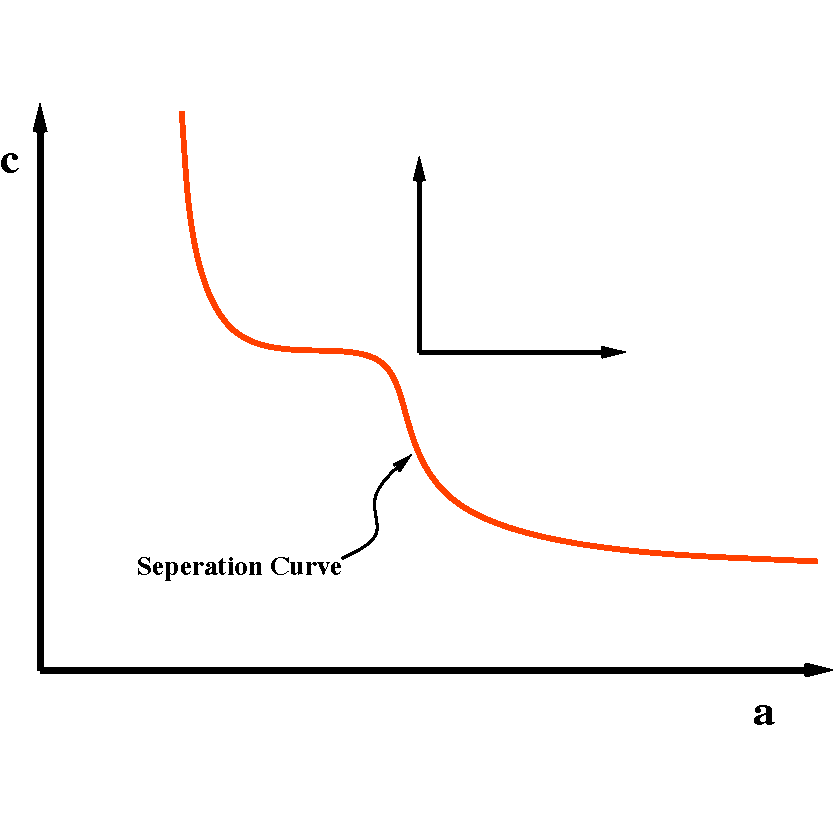
\includegraphics[height=5cm]{figures/achievable1.pdf}
\end{center}
\end{itemize}
\end{frame}

\section{Analysis for specific loss functions}

\begin{frame}
\frametitle{Analysis for specific loss functions}
\begin{itemize}
\item
\B{Outcomes:} \R{$\omega^1,\omega_2,\ldots$ $\omega^t \in [0,1]$}  
\item
\B{Predictions:} \R{$\gamma^1,\gamma^2,\ldots$  $\gamma^t \in [0,1]$}
\end{itemize}
\end{frame}

\begin{frame}
\frametitle{Log loss (Entropy loss)} 
\begin{itemize}
\item
\R{\[ \lambda_{\text{ent}}(\omega,\gamma) = \omega \ln \frac{\omega}{\gamma} 
                              +(1-\omega) \ln \frac{1-\omega}{1-\gamma} \]}
\item
When \R{$q_t \in \{0,1\}$} Cumulative log loss \R{$=$} coding length \R{$\pm 1$}
\item
If \R{$P[\omega_t=1]=q$}, optimal prediction \R{$\gamma^t=q$}
\item
\B{Un}bounded loss.
\item
\B{Not} symmetric \R{$\exists p,q\;\; \lambda(p,q) \neq \lambda(q,p)$}.
\item
\B{No} triangle inequality
\R{$ \exists p_1,p_2,p_3\;\; \lambda(p_1,p_3) > \lambda(p_1,p_2) + \lambda(p_2,p_3)$}
\end{itemize}
\end{frame}

\begin{frame}
\frametitle{Square loss (Breier Loss)}
\begin{itemize}
\item
\R{\[ \lambda_{\text{sq}}(\omega,\gamma)  = (\omega-\gamma)^2 \]}
\item
\R{$P[\omega^t=1]=q,\;\; P[\omega^t=0]=1-q$}, \\
optimal prediction \R{$\gamma^t=q$}
\item
Bounded loss.
\item
Defines a metric (symmetric and triangle ineq.)
\item
Corresponds to regression.
\end{itemize}
\end{frame}

\begin{frame}
\frametitle{Hellinger Loss}

\begin{itemize}
\item
\R{\[ \lambda_{\text{hel}}(\omega,\gamma)  = \frac{1}{2} \paren{
\paren{\sqrt{\omega} +\sqrt{\gamma}}^2 + 
\paren{\sqrt{1-\omega}+\sqrt{1-\gamma}}^2 
} \] } 
\item
If \R{$P[\omega^t=1]=q,\;\; P[\omega^t=0]=1-q$}, \\
optimal prediction \R{$\gamma^t=q$}
\item
Loss is bounded.
\item
Defines a metric.
\item 
\R{$\lambda_{\text{hel}}(p,q)  \approx \lambda_{\text{ent}}(p,q)$} when 
\R{$p \approx q$} and \R{$p,q \in (0,1)$}
\end{itemize}
\end{frame}

\begin{frame}
\frametitle{Absolute loss}

\begin{itemize}
\item
\R{\[ \lambda(\omega,\gamma) = | \omega -\gamma | \]}
\item
Probability of making a mistake if predicting 0 or 1 
using a biased coin\\
\item
If \R{$P[\omega^t=1]=q,\;\; P[\omega^t=0]=1-q$}, then the optimal prediction is 
\R{\[
\gamma^t = 
\begin{cases} 1 & \text{if $q>1/2$,} \\
              0 & \text{otherwise}
\end{cases}
\]}
\end{itemize}
\end{frame}

\begin{frame}
\frametitle{Structureless bounded loss}

\begin{itemize}
\item Prediction is a distribution 
\R{$\gamma = \langle p_1,\ldots,p_N \rangle$, $p_i \geq 0$, $\sum_{i=1}^N p_i = 1$}
\item Outcome is a loss vector \R{$\omega = \langle \omega_1,\ldots,\omega_N \rangle$, 
$0 \leq \omega_i \leq 1$}
\item Loss is the dot product: \R{$\lambda_{\text{dot}}(\omega,\gamma) = \gamma \cdot \omega$}
\item Corresponds to the hedging game.
\item For hedge loss the regret is \R{$\Omega(\sqrt{T \log N})$}.
\item For the log loss the regret is \R{$O(\log N)$}
\item {\bf Which losses behave like \B{entropy loss} and which behave like \B{hedge loss}}?
\end{itemize}
\end{frame}


\begin{frame}
\frametitle{Some technical requirements}
\begin{itemize}
\item There should be a \B{topology} on the prediction set \R{$\Gamma$} such that
\item
\R{$\Gamma$} is compact.
\item
\R{$\forall \omega \in \Omega$}, the function 
\R{$\gamma \to \lambda(\omega,\gamma)$} is \B{continuous}
\item
There is a \B{universally reasonable prediction} \\
\R{$\exists \gamma \in \Gamma$, $\forall \omega \in \Omega$,
$\lambda(\omega,\gamma) < \infty$}
\item
There is \B{no universally optimal prediction} \\
\R{$\neg \exists \gamma \in \Gamma$, $\forall \omega \in \Omega$,
$\lambda(\omega,\gamma) = 0$}
\end{itemize}
\end{frame}

\section{Vovk's algorithm}

\begin{frame}
\frametitle{Vovk's meta-algorithm}
\begin{itemize}
\item Fix an \B{achievable} pair \R{$(a,c)$} and set \R{$\eta=a/c$}
\item \begin{enumerate}
\item
\R{$$
	\weight{i}{t} = {1 \over N} \; e^{-\eta \TEloss{i}^{t}}
$$}
\item
Choose $\gamma_t$ so that, for all $\omega^t \in \Omega$:
\R{\[
\lambda(\omega^t,\gamma^t) - c \ln \sum_i \weight{i}{t} 
\leq
- c \ln \left( \sum_i 
      \weight{i}{t}e^{-\eta \lambda(\omega^t,\gamma_i^t)}
        \right)
\]}
\end{enumerate}
\item
If choice of \R{$\gamma_t$} always exists, then the total loss satisfies:
\R{\[
\sum_t \lambda(\omega^t,\gamma^t)
\leq
- c \ln \sum_i \weight{i}{T+1}
\leq
a \BEloss + c \ln N
\]}
\item
Vovk's result: \B{\em yes!} a good choice for \R{$\gamma_t$} always exists!
\end{itemize}
\end{frame}

\begin{frame}
\frametitle{Vovk's algorithm is the the highest achiever {\color{green} [Vovk95]}}

The pair \R{$(a,c)$} is achieved by \B{some} algorithm 
if and only if it is achieved by \B{Vovk's} algorithm.
\pause \\
The separation curve is
\R{$ \left\{ \left. \left( a(\eta),{a(\eta) \over \eta} \right) \right| 
           \eta \in [0,\infty] \right\} $}
\pause
\begin{center}
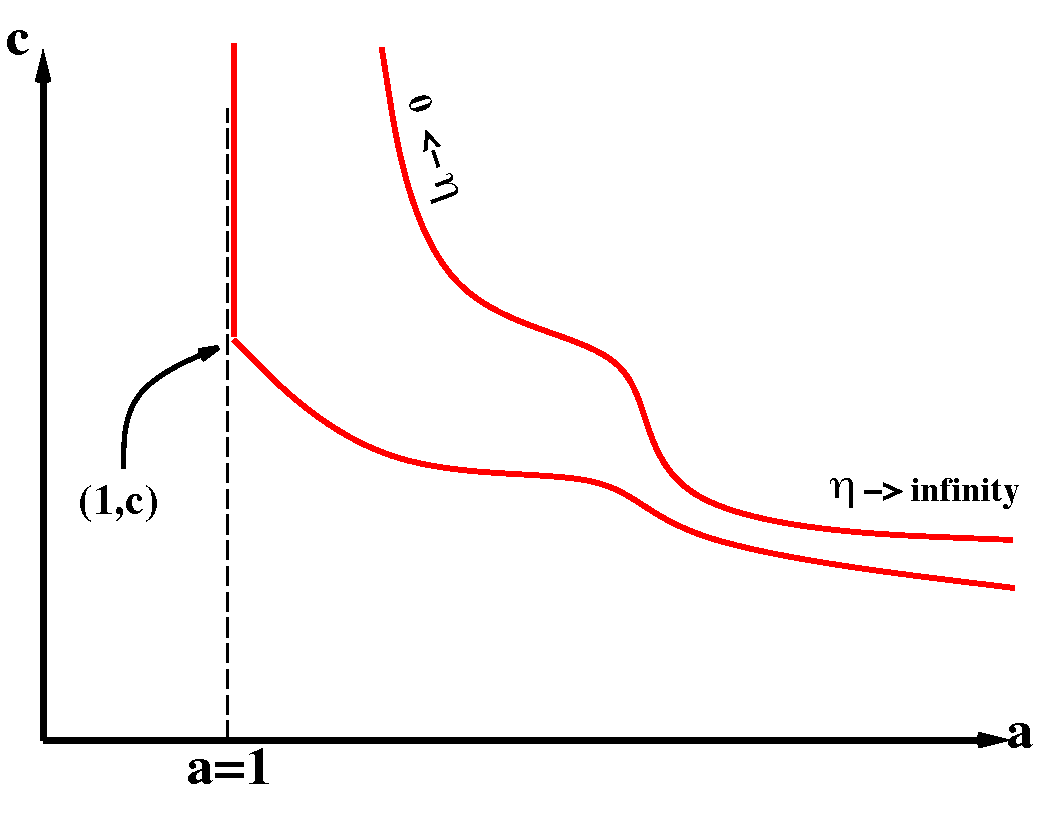
\includegraphics[height=5cm]{figures/achievable2.pdf}
\end{center}
\end{frame}

\section{mixable loss functions}
\begin{frame}
\frametitle{Mixable Loss Functions}
\begin{itemize}
\item A Loss function is \B{mixable} if a pair of the form \R{$(1,c),\; c<\infty$} is achievable.
\R{\[
\TAloss \leq \BEloss + c \ln N 
\]}
\item Vovk's algorithm with \R{$\eta = 1/c$} achieves this bound.
\item \R{$\lambda_{\text{ent}},\lambda_{\text{sq}},\lambda_{\text{hel}}$} are \B{mixable}
\item \R{$\lambda_{\text{abs}},\lambda_{\text{dot}}$} are \B{not mixable}
\end{itemize}
\end{frame}


\section{The convexity condition}

\begin{frame}
\frametitle{The convexity condition}
\begin{itemize}
\item requirement for loss to be \R{$(1,1/\eta)$} mixable
\item 
\R{$\forall \langle (\gamma_1,\weight{1}{}),\ldots,(\gamma_N,\weight{N}{}) \rangle$} \\
\R{$\exists \B{\gamma} \in \Gamma$} \\
\R{$\forall \omega \in \Omega$}:
\R{\[
\lambda(\omega,\B{\gamma}) - \frac{1}{\eta} \ln \sum_i \weight{i}{} 
\leq
- \frac{1}{\eta} \ln \left( \sum_i 
      \weight{i}{}e^{-\eta \lambda(\omega,\gamma_i)}
        \right)
\]}
\item
Can be re-written as:
\R{\[
e^{-\eta \lambda(\omega,\B{\gamma})}
\geq
\sum_i 
\left({\weight{i}{} \over \sum_j \weight{j}{}}\right)
e^{-\eta \lambda(\omega,\gamma_i)}
\]}
%% \item \B{Assumption:}
%% fix \R{$\lambda(\omega,\gamma_i)$} for all but \R{$i \not\in \{j,k\}$}
%% then increasing \R{$\lambda(\omega,\gamma_j)$} decreases
%% \R{$\lambda(\omega,\gamma_k)$}
\item
Equivalently - the image of the set \R{$\Gamma$} under the
mapping
\R{$F(\gamma) = 
\left\langle 
   e^{-\eta \lambda(\omega,\gamma)} 
\right\rangle_{\omega \in \Omega}
$} is concave.
\end{itemize}
\end{frame}

\begin{frame}
\frametitle{convexity condition: Pictorially}
\begin{itemize}
\item
\noindent {\bf Example:} Suppose $\Omega=\{0,1\}$, $\Gamma = [0,1]$.
then
\[
F(\gamma) = \left\langle
  e^{-\eta \lambda(0,\gamma)},e^{-\eta \lambda(1,\gamma)}
\right\rangle
\]
\item
\begin{center}
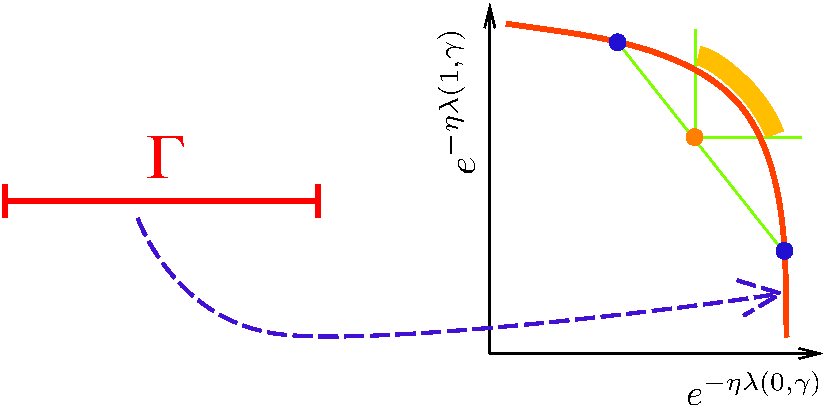
\includegraphics[height=5cm]{figures/convex.pdf}
\end{center}
\end{itemize}
\end{frame}

\section{Log loss}

\begin{frame}
\frametitle{Vovk Algorithm for log loss}
\begin{itemize}
\item The log loss is mixable with \R{$\eta=1$}
\item The image of \R{$[0,1]$} through \R{$F(\gamma) = \left\langle
  e^{-\eta \lambda(0,\gamma)},e^{-\eta \lambda(1,\gamma)} \right\rangle$} is a straight line segment.
\item The \B{only} satisfactory prediction is 
\R{\[
\gamma = \frac{\sum_i \weight{i}{} \gamma_i}{\sum_i \weight{i}{}}
\]}
\item
We are back to the online Bayes algorithm.
\end{itemize}
\end{frame}

\section{Square loss}

\begin{frame}
\frametitle{Vovk algorithm for square loss}
\begin{itemize}
\item The square loss is mixable with $\eta=2$.
\item Prediction must satisfy
\R{\[
1-\sqrt{ -{1 \over 2} \ln \sum_i \Nweight{i}{t} e^{-2(1-p^t_i)^2} }
\leq
p^t
\leq
\sqrt{ -{1 \over 2} \ln \sum_i \Nweight{i}{t} e^{-2(p^t_i)^2} }
\]}
where
\R{$
	\Nweight{i}{t} = {\weight{i}{t} \over \sum_s \weight{i}{s}}~.
$}
\item
\R{$$ \TAloss \leq \BEloss + \frac{1}{2}\ln N $$}
\end{itemize}
\end{frame}

\subsection{Square loss using simple averaging}

\begin{frame}
\frametitle{Simple prediction for square loss}
\begin{itemize}
\item We can use the prediction
\R{\[
\gamma = \frac{\sum_i \weight{i}{} \gamma_i}{\sum_i \weight{i}{}}
\]}
\item But in that case we must use \R{$\eta=1/2$} when updating the weights.
\item Which yields the bound
\R{$$ \TAloss \leq \BEloss + 2 \ln N $$}
\end{itemize}
\end{frame}

\section{Summary table}

\begin{frame}
\frametitle{Summary of bounds for mixable losses}
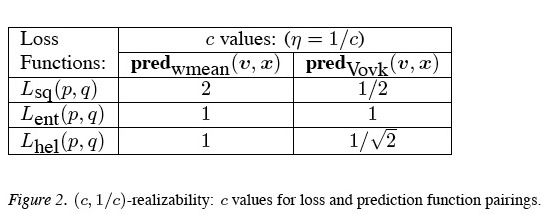
\includegraphics[height=6cm]{figures/summarytable.jpg}
\end{frame}

\endgroup
\iffalse %%%%%%%%%%%%%%%%%%%%%%%%%%%%%%%%%%%%%%%%%%%%%%%%%%%%%%%%%%%%%%%%%%

\fi %%%%%%%%%%%%%%%%%%%%%%%%%%%%%%%%%%

\end{document}


